\subsection{Протокол Yahalom}\index{протокол!Yahalom|(}\label{section-protocols-yahalom}

Протокол Yahalom можно рассматривать как улучшенную версию протокола Wide-Mouth Frog\index{протокол!Wide-Mouth Frog} из раздела~\ref{section-protocols-wide-moth-frog}. Данный протокол <<перекладывает>> генерацию нового сессионного ключа на сторону доверенного центра, а также использует случайные числа в качестве попыток защиты от атак повтором.

\begin{figure}[!htb]
    \centering
    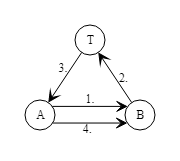
\includegraphics[width=0.5\textwidth]{pic/key_distribution-yahalom}
    \caption{Схема взаимодействия абонентов и доверенного центра в протоколе Yahalom\label{fig:key_distribution-yahalom}}
\end{figure}

\begin{samepage}\begin{itemize}
	\item[(1)] $Alice \to \{ A, R_A \} \to Bob$
	\item[(2)] $Bob \to \{ B, E_B( A, R_A, R_B ) \} \to Trent$
	\item[(3)] Трент генерирует новый сессионный ключ $K$
	\item[{}] $Trent \to \{ E_A( B, K, R_A, R_B ), E_B(A, K) \} \to Alice$
	\item[(4)] $Alice \to \{ E_B( A, K ), E_K( R_B ) \} \to Bob$
\end{itemize}\end{samepage}

После того, как Боб провалидирует число $R_B$, присланное Алисой, стороны смогут использовать новый сессионный ключ $K$. Протокол, кроме генерации ключа, обеспечивает взаимную аутентификацию сторон:

\begin{itemize}
    \item Аутентификация Алисы перед Бобом происходит на 4-м проходе, когда Боб может провалидировать возможность Алисы зашифровать известное только ей (и Тренту) случайное число $R_B$ на ключе $K$.
    \item Аутентификация Боба перед Алисой происходит на 3-м проходе, когда Трент демонстрирует Алисе, что он получил случайное число $R_A$ именно от Боба.
\end{itemize}

Хотя Боб сумел доказать Тренту, что он является Бобом, а Трент, в свою очередь, продемонстрировал это Алисе, нужно отметить (\cite{Zhou:Yu:Pan:Wang:2016}), что в рамках протокола Боб никак не доказал, что он получил новый сессионный ключ и может им оперировать. Также на 3-м проходе Трент не включает случайное число $R_B$ в сообщение $E_B(A, K)$, что позволяет Алисе, действуя не из лучших побуждений, заставить Боба принять старый сессионный ключ.

\begin{samepage}\begin{itemize}
	\item[(1)] $Alice \to \{ A, R_A \} \to Bob$
	\item[(2)] $Bob \to \{ B, E_B( A, R_A, R_B ) \} \to Trent$
	\item[(3)] Трент генерирует новый сессионный ключ $K$
	\item[{}] $Trent \to \{ E_A( B, K, R_A, R_B ), E_B(A, K) \} \to Alice$
	\item[(4)] Алиса использует старый сессионный ключ $K^*$ и сообщение $E_B( A, K^* )$ из старого сеанса протокола
	\item[{}] $Alice \to \{ E_B( A, K^* ), E_{K^*}( R_B ) \} \to Bob$
\end{itemize}\end{samepage}

Протокол Yahalom послужил основной большому количеству научных работ, связанных с автоматизированным анализом стойкости криптографических протоколов и имел несколько <<улучшенных>> вариантов. Однако о широком использовании данного протокола в реальных информационных системах неизвестно.

\index{протокол!Yahalom|)}
